% ----------------------------------
% Cap Captura de Requisitos
% ----------------------------------
%	A MEJORAR - 
%		Hay que desarrollar mucho más cada una de las interfaces y colocar mejor las imágenes
%		Aunque esté en el Análisis, el diseño de interfaces pertenece a la fase de diseño
%

\chapter{Análisis} % (fold)
	\label{cha:analisis}

% 
% Sec Tipos de usuarios
%
\section{Modelo de casos de uso} % (fold)
	\label{sec:modelo_casos_de_uso}
	
% section modelo_de_casos_de_uso (end)

%
% Sec Diseño de interfaz de usuario
%
\section{Diseño de interfaz de usuario} % (fold)
	\label{sec:diseno_de_interfaz_de_usuario}

	Se realiza una primera aproximación a lo que será la interfaz de usuario que se implementará para la aplicación. Se cuenta con una interfaz pública para los entrenadores que acceden a la web, donde pueden ver las referencias y tour de la aplicación. Por otro lado, están detalladas las interfaces de cada uno de los módulos que proporcionan las funcionalidades a los entrenadores registrados.
	
	\begin{figure}[H]
	  \centering
	    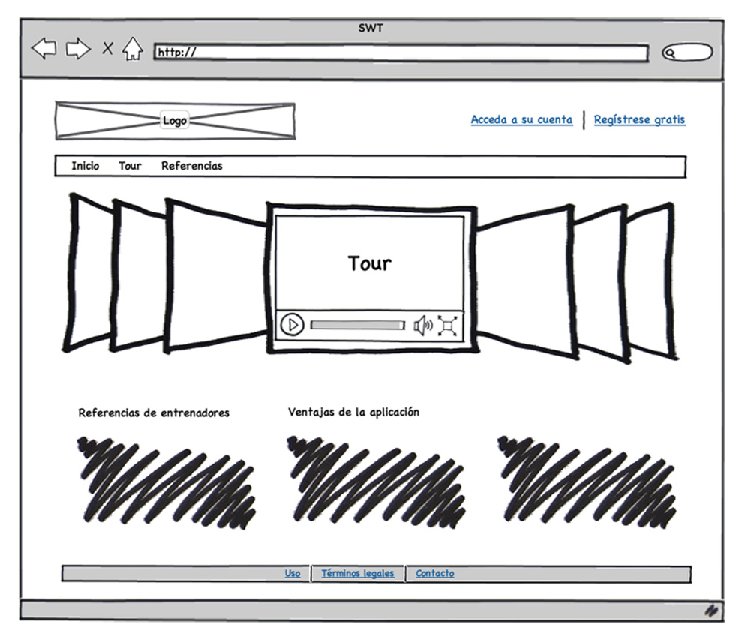
\includegraphics[width=8cm]{./eps/1_Inicio.eps}
	  \caption{Inicio en la interfaz pública}
	  \label{fig:interfaz_publica_inicio}
	\end{figure}
	
	\subsection{Interfaz pública} % (fold)
		\label{sub:interfaz_publica}
		
		La figura \ref{fig:interfaz_publica_inicio} muestra la estructura de la página web que actúa como interfaz pública. La parte superior está compuesta por el logo, enlace a registro/acceso a la aplicación y un menú para acceder al resto de páginas públicas a los entrenadores que aún no estén registrados en el sistema.
			
		El resto de interfaces públicas que la conforman son: {\it tour} con las características y ventajas del sistema (figura \ref{fig:interfaz_publica_tour}); {\it referencias} de los entrenadores que participan en la elaboración del proyecto; página de {\it contacto} (figura \ref{fig:interfaz_publica_contacto}) con los administradores; {\it términos legales y de uso}. 
		
		\begin{figure}[H]
		  \centering
		    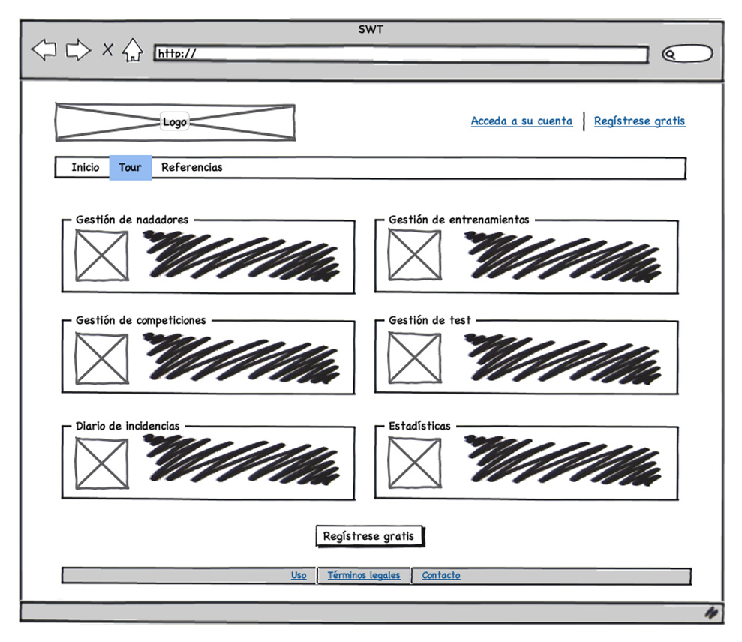
\includegraphics[width=8cm]{./eps/2_Tour.eps}
		  \caption{Tour en la interfaz pública}
		  \label{fig:interfaz_publica_tour}
		\end{figure}

		\begin{figure}[H]
		  \centering
		    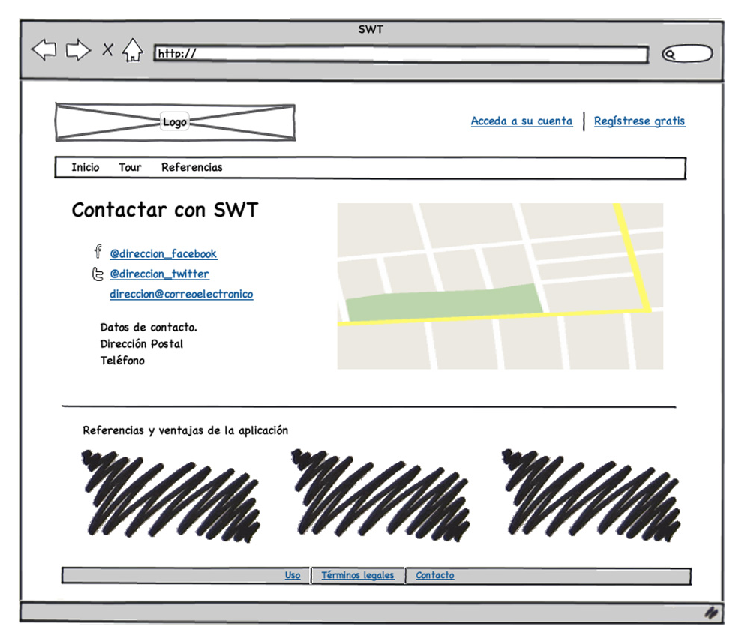
\includegraphics[width=8cm]{./eps/3_Contacto.eps}
		  \caption{Contacto en la interfaz pública}
		  \label{fig:interfaz_publica_contacto}
		\end{figure}

	% subsection interfaz_pública (end)
	
	\subsection{Registro y acceso} % (fold)
		\label{sub:registro_y_acceso}
	
		Las interfaces para el registro (figura \ref{fig:interfaz_registro}) y acceso (figura \ref{fig:interfaz_acceso}) de un entrenador al sistema son muy similares. Su estructura es algo diferente al resto de páginas de la aplicación, eliminando elementos que puedan interferir en el objetivo último ---registrarse o acceder. Hay que destacar que para el acceso, el identificador de usuario viene proporcionado por el correo electrónico insertado en la fase de registro.
		
		\begin{figure}[H]
		  \centering
		    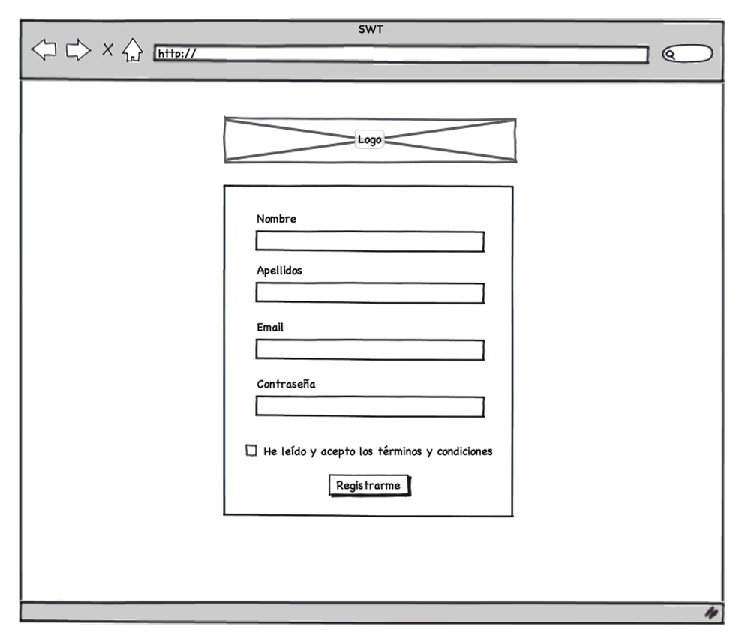
\includegraphics[width=8cm]{./eps/4_Registro.eps}
		  \caption{Interfaz para el registro de un entrenador}
		  \label{fig:interfaz_registro}
		\end{figure}
		
		\begin{figure}[H]
		  \centering
		    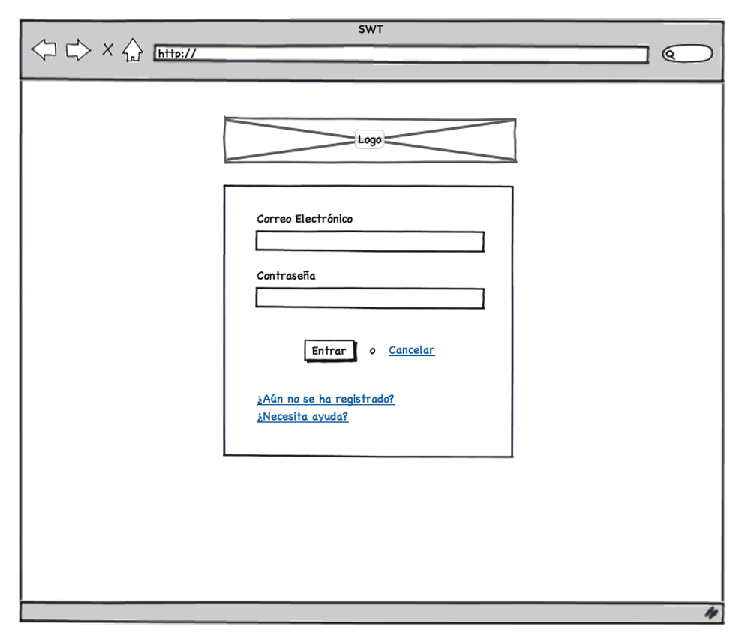
\includegraphics[width=8cm]{./eps/5_Acceder.eps}
		  \caption{Interfaz para el acceso de un entrenador}
		  \label{fig:interfaz_acceso}
		\end{figure}
	% subsection registro_y_acceso (end)
	
	\subsection{Dashboard} % (fold)
		\label{sub:interfaz_dashboard}
	
	Cuando el entrenador se registra en la aplicación, la primera página a la que accede es la de {\it dashboard} o resumen (figura \ref{fig:interfaz_dashboard}). En ella, lo primero que aparece es un recordatorio de los pasos que tiene que hacer para empezar a sacar provecho de la aplicación. A diferencia de las páginas vistas hasta el momento, ésta incluye en su estructura una barra lateral con los accesos que más frecuentemente se usan.
		
		\begin{figure}[H]
		  \centering
		    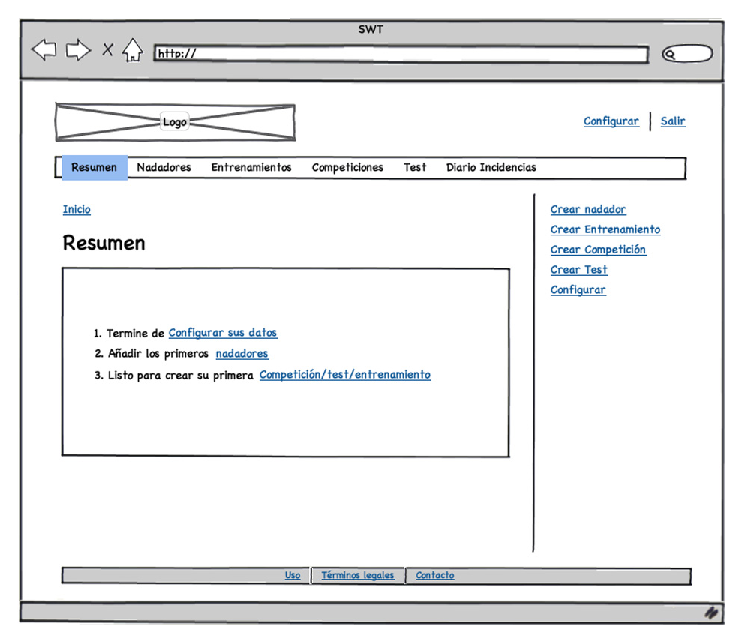
\includegraphics[width=8cm]{./eps/6_Dashboard.eps}
		  \caption{Interfaz para el dashboard de un entrenador}
		  \label{fig:interfaz_dashboard}
		\end{figure}
		
	% subsection dashboard (end)
	
	\subsection{Configuración del perfil} % (fold)
		\label{sub:configuracion_del_perfil}
	
	Cada entrenador registrado tiene un perfil asociado, donde se guarda información del tipo personal (figura \ref{fig:interfaz_conf_personal}), de contacto (figura \ref{fig:interfaz_conf_contacto}) y los parámetros relacionados con el índice de Mujika (figura \ref{fig:interfaz_conf_mujika}). La información está estructurada en pestañas para una mayor facilidad de navegación.
	
		\begin{figure}[H]
		  \centering
		    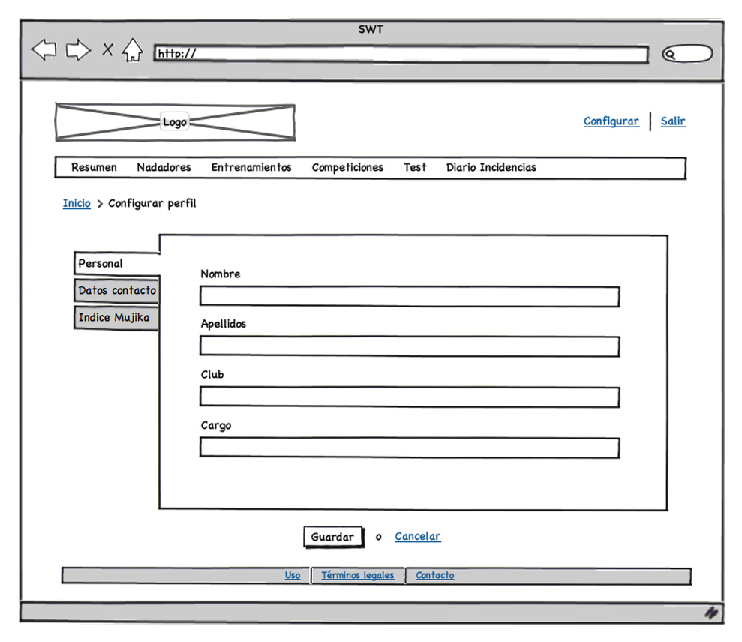
\includegraphics[width=8cm]{./eps/7_Conf_personal.eps}
		  \caption{Interfaz para la configuración de la información personal en el perfil}
		  \label{fig:interfaz_conf_personal}
		\end{figure}
		
		\begin{figure}[H]
		  \centering
		    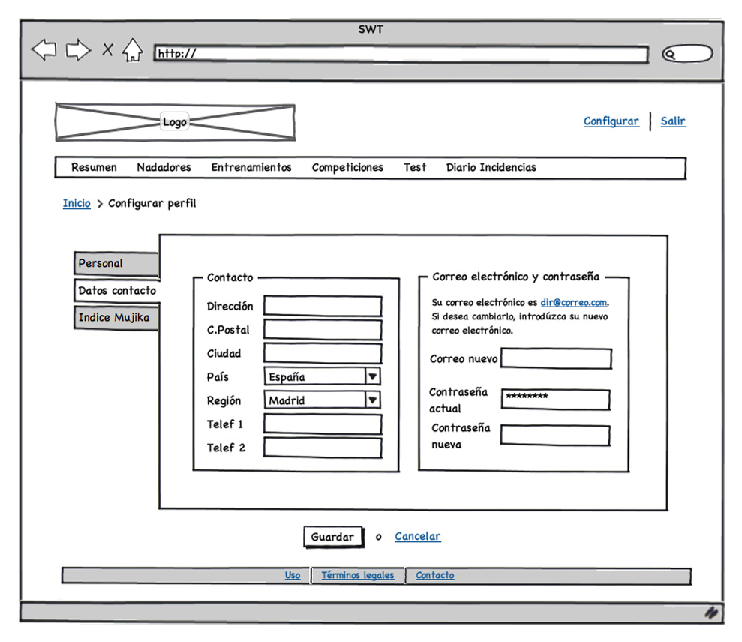
\includegraphics[width=8cm]{./eps/8_Conf_contacto.eps}
		  \caption{Interfaz para la configuración de la información de contacto en el perfil}
		  \label{fig:interfaz_conf_contacto}
		\end{figure}
		
		\begin{figure}[H]
		  \centering
		    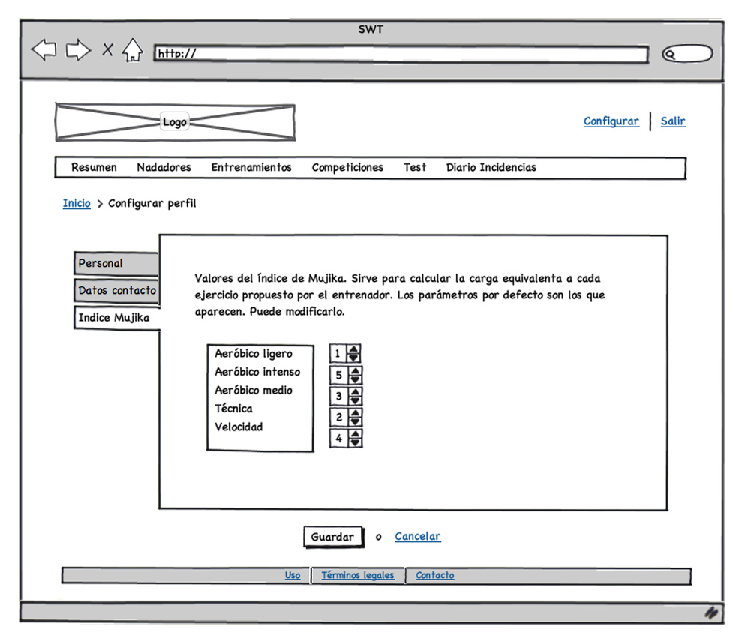
\includegraphics[width=8cm]{./eps/9_Conf_mujika.eps}
		  \caption{Interfaz para la configuración del índice de Mujika en el perfil}
		  \label{fig:interfaz_conf_mujika}
		\end{figure}
		
	% subsection configuración_del_perfil (end)
	
	\subsection{Gestión de nadadores} % (fold)
		\label{sub:gestion_de_nadadores}
	
	Uno de los módulos fundamentales en la aplicación es el de gestión de nadadores. Es, en gran medida, la base para las competiciones y los test, puesto que los resultados que se insertan en ellos dependen de los nadadores que un entrenador maneja. 
	
	La estructura de la interfaz es común al resto de módulos y está compuesta de:
		
	\begin{itemize}
		\item {{\bf Tabla}. Muestra los registros insertados por un entrenador pertenecientes al módulo en que se encuentre. En este caso, como se está en la sección de nadadores, aparece el conjunto de nadadores que el entrenador ha dado de alta en el sistema.}
		\item {{\bf Buscador}. Campo de búsqueda que localiza registros por diferentes parámetros.}
		\item {{\bf Resumen}. Muestra información relevante al módulo en que se encuentre. Lo normal es que aparezca el número de registros insertados en cada módulo.}
		\item {{\bf Barra lateral}. Desde ella se accede a cada una de las opciones del módulo que se esté gestionando.}
	\end{itemize}
	
	A continuación se muestran las interfaces de {\it ver listado de nadadores} (figura \ref{fig:interfaz_nadadores}), {\it añadir nadador} (figura \ref{fig:interfaz_nadadores_new}), {\it ver nadador} (figura \ref{fig:interfaz_nadadores_show}) y {\it modificar nadador} (figura \ref{fig:interfaz_nadadores_modif}). La primera de ellas muestra todos los nadadores insertados en la aplicación por un entrenador registrado; la segunda refleja el proceso para añadir un nuevo nadador; y la tercera como se modificaría. Es destacable que la información relacionada con las competiciones y test que aparece en {\it ver nadador}, no pueden ser modificadas desde este módulo, sino desde los que gestionan las competiciones y test.
	
	\begin{figure}[H]
	  \centering
	    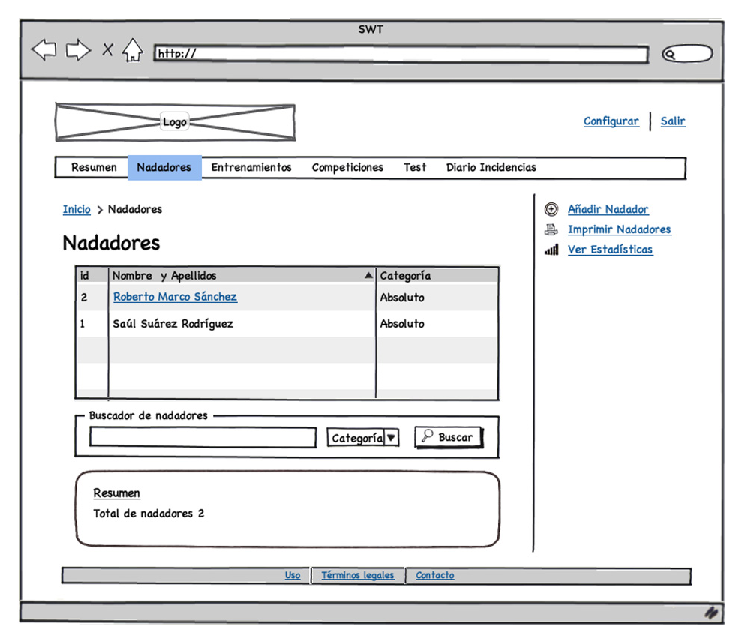
\includegraphics[width=8cm]{./eps/10_Nadadores.eps}
	  \caption{Interfaz para ver listado de nadadores}
	  \label{fig:interfaz_nadadores}
	\end{figure}
	
	\begin{figure}[H]
	  \centering
	    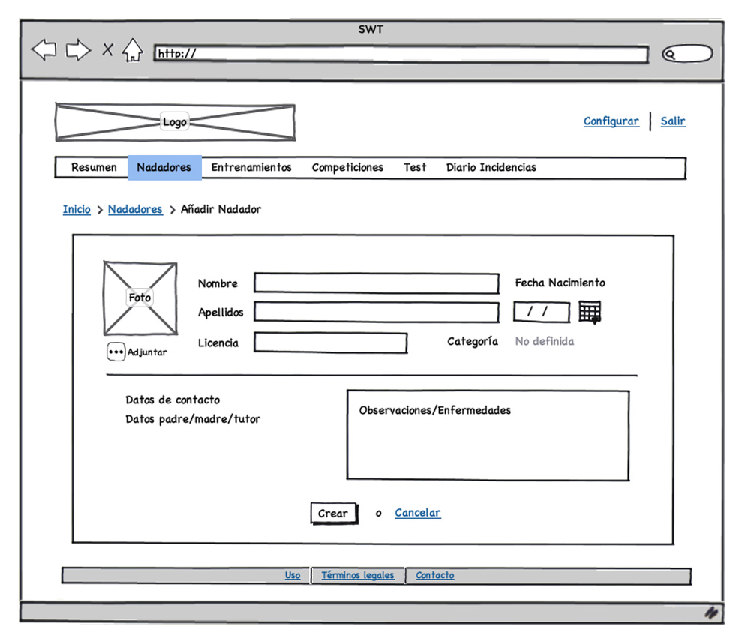
\includegraphics[width=8cm]{./eps/11_Nadadores_new.eps}
	  \caption{Interfaz para añadir nadador}
	  \label{fig:interfaz_nadadores_new}
	\end{figure}
	
	\begin{figure}[H]
	  \centering
	    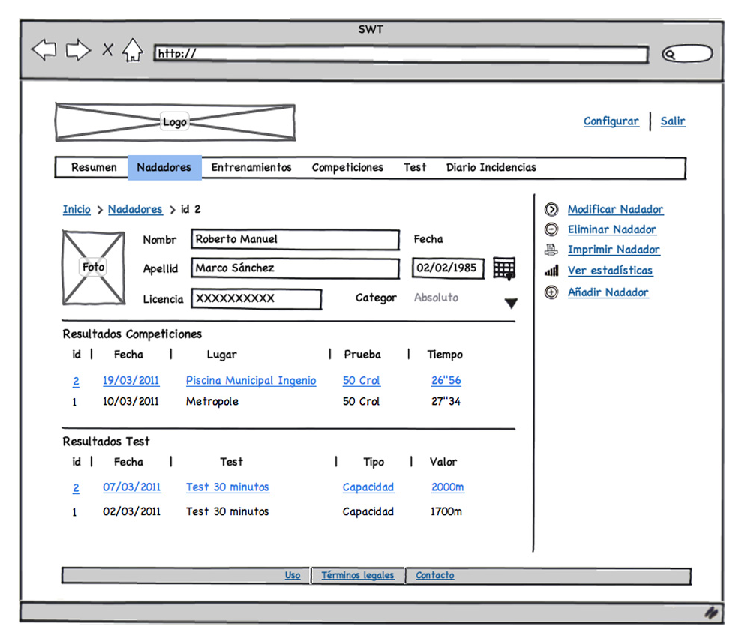
\includegraphics[width=8cm]{./eps/12_Nadadores_show.eps}
	  \caption{Interfaz para ver nadador}
	  \label{fig:interfaz_nadadores_show}
	\end{figure}
	
	\begin{figure}[H]
	  \centering
	    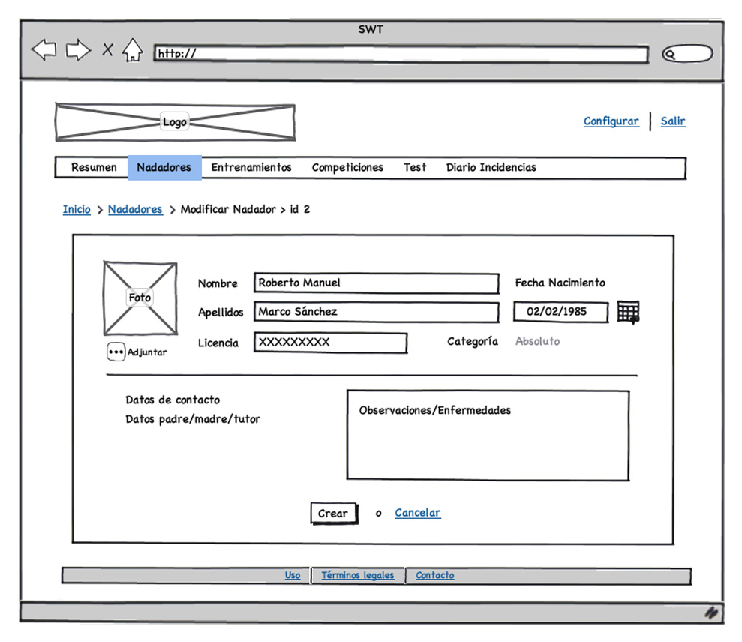
\includegraphics[width=8cm]{./eps/13_Nadadores_modif.eps}
	  \caption{Interfaz para modificar nadador}
	  \label{fig:interfaz_nadadores_modif}
	\end{figure}
	% subsection gestión_de_nadadores (end)
	
	\subsection{Gestión de Competiciones} % (fold)
		\label{sub:gestion_de_competiciones}
	
	La figura \ref{fig:interfaz_competiciones} muestra la interfaz para ver las competiciones añadidas por un entrenador registrado. Su estructura, como se especificó anteriormente, es similar a la del resto de módulos. La particularidad que tiene es que aparece un calendario de la temporada. A medida que se {\it añadan competiciones} (figura \ref{fig:interfaz_competiciones_new}) irán apareciendo ahí. 
	
		\begin{figure}[H]
		  \centering
		    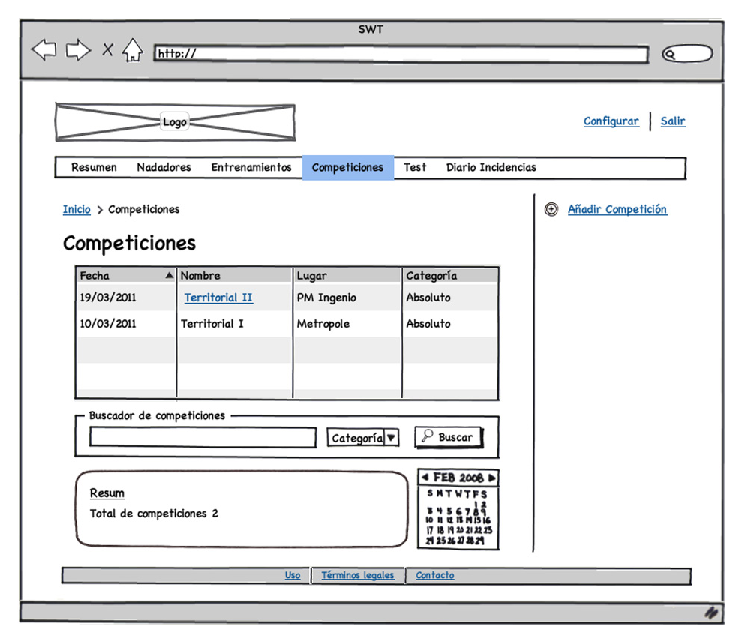
\includegraphics[width=8cm]{./eps/14_Competiciones.eps}
		  \caption{Interfaz para ver listado de competiciones}
		  \label{fig:interfaz_competiciones}
		\end{figure}

		\begin{figure}[H]
		  \centering
		    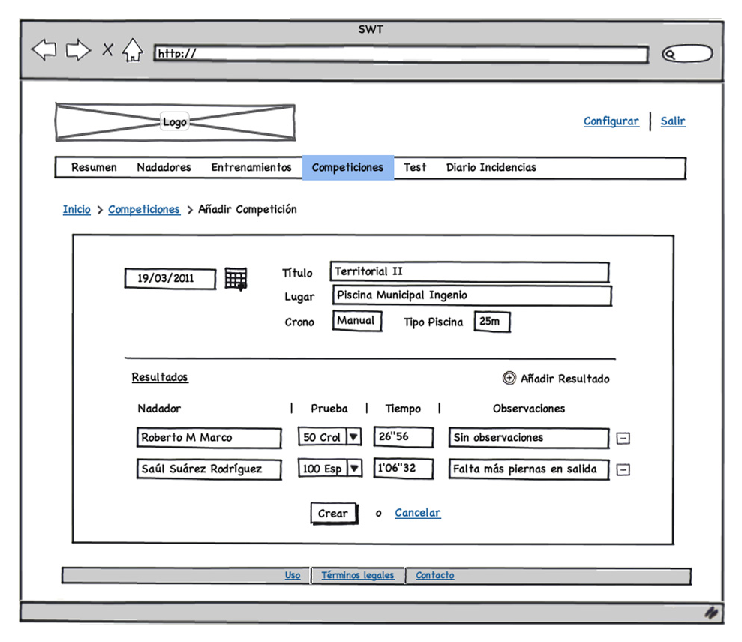
\includegraphics[width=8cm]{./eps/15_Competiciones_new.eps}
		  \caption{Interfaz para añadir competición}
		  \label{fig:interfaz_competiciones_new}
		\end{figure}

Cuando un entrenador hace clic sobre el nombre de la competición en la tabla, se accede a {\it ver una competición} (figura \ref{fig:interfaz_competiciones_show}). Cuando se modifica una competición (figura \ref{fig:interfaz_competiciones_modif}), se da la posibilidad de modificar cada uno de los resultados añadidos a la misma. Esta información es la que aparecerá modificada en la ficha de cada nadador.

		\begin{figure}[H]
		  \centering
		    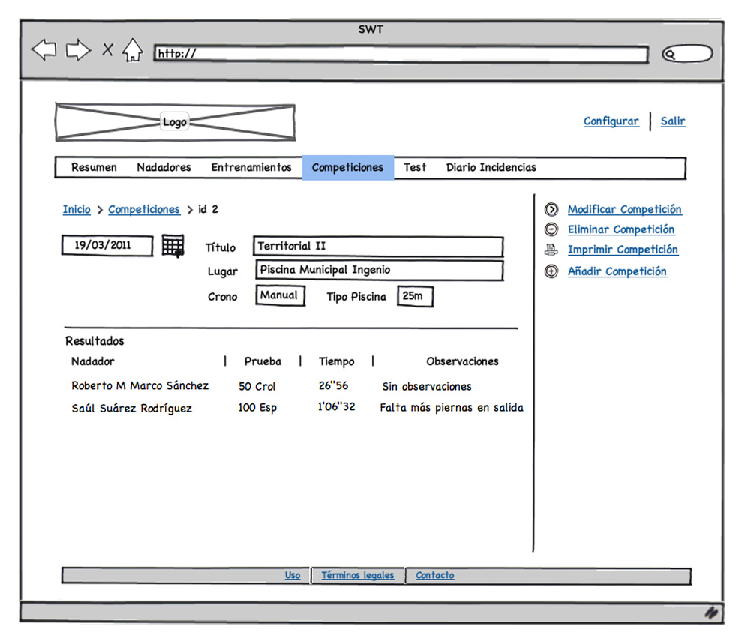
\includegraphics[width=8cm]{./eps/16_Competiciones_show.eps}
		  \caption{Interfaz para ver competición}
		  \label{fig:interfaz_competiciones_show}
		\end{figure}

		\begin{figure}[H]
		  \centering
		    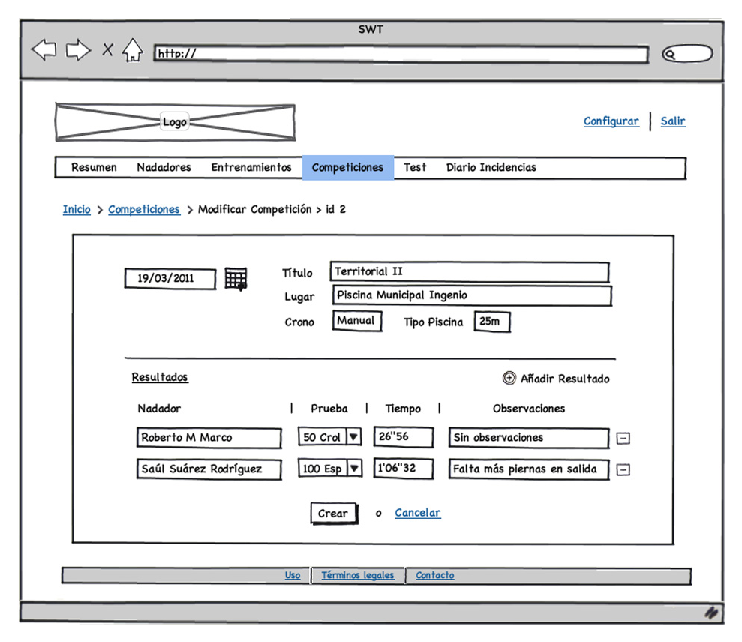
\includegraphics[width=8cm]{./eps/17_Competiciones_modif.eps}
		  \caption{Interfaz para modificar competición}
		  \label{fig:interfaz_competiciones_modif}
		\end{figure}
	% subsection gestión_de_competiciones (end)
	
	\subsection{Gestión de entrenamientos} % (fold)
		\label{sub:gestion_de_entrenamientos}
	
	La {\it lista de entrenamientos} (figura \ref{fig:interfaz_entrenamientos}) refleja cada una de las sesiones que inserta el entrenador a lo largo de una temporada. En el resumen se muestran la cantidad de sesiones, el volumen y la carga realizadas en total. Al hacer clic sobre el nombre del entrenamiento, se accede a {\it ver entrenamiento} (figura \ref{fig:interfaz_entrenamientos_show}), que incluye cada uno de los ejercicios añadidos al mismo. Como cada ejercicio tiene asociado un volumen y una carga, se muestra el total de esa sesión. Esto ayuda al entrenador a la hora de hacer los entrenamientos, puesto que conoce el estado a medida que los va desarrollando.
	Añadir (figura \ref{fig:interfaz_entrenamientos_new}) y modificar entrenamiento son iguales, con la salvedad de que el segundo permite cambiar los datos de los formularios que se agregan en el primero.
	
	\begin{figure}[H]
	  \centering
	    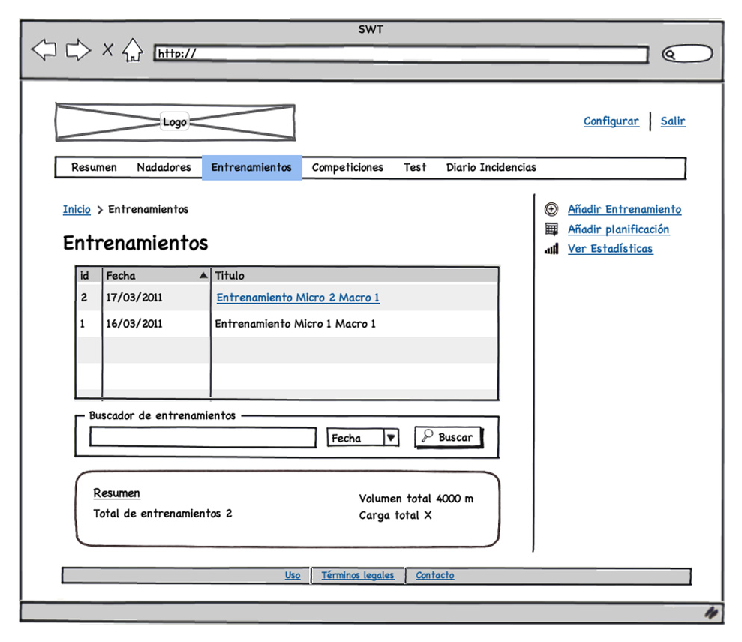
\includegraphics[width=8cm]{./eps/18_Entrenamientos.eps}
	  \caption{Interfaz para ver listado de entrenamientos}
	  \label{fig:interfaz_entrenamientos}
	\end{figure}

	\begin{figure}[H]
	  \centering
	    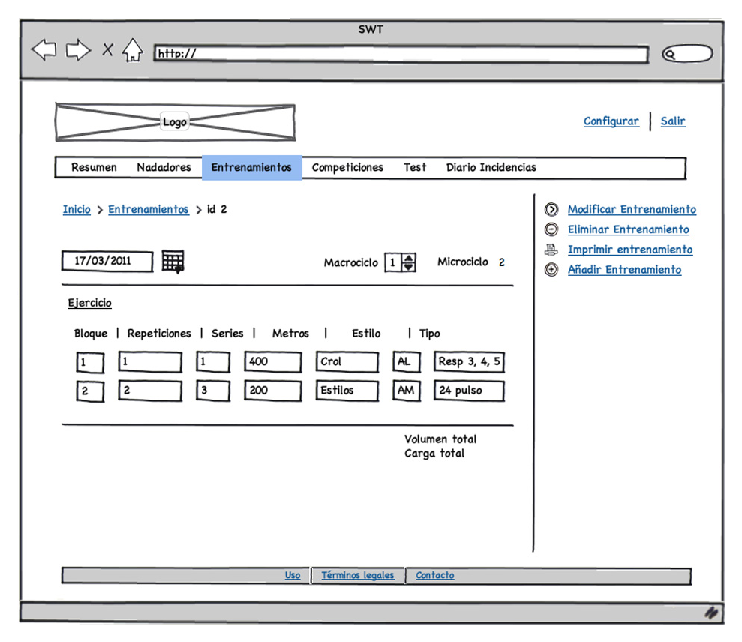
\includegraphics[width=8cm]{./eps/20_Entrenamientos_show.eps}
	  \caption{Interfaz para ver entrenamiento}
	  \label{fig:interfaz_competiciones_show}
	\end{figure}
	
	
	
	\begin{figure}[H]
	  \centering
	    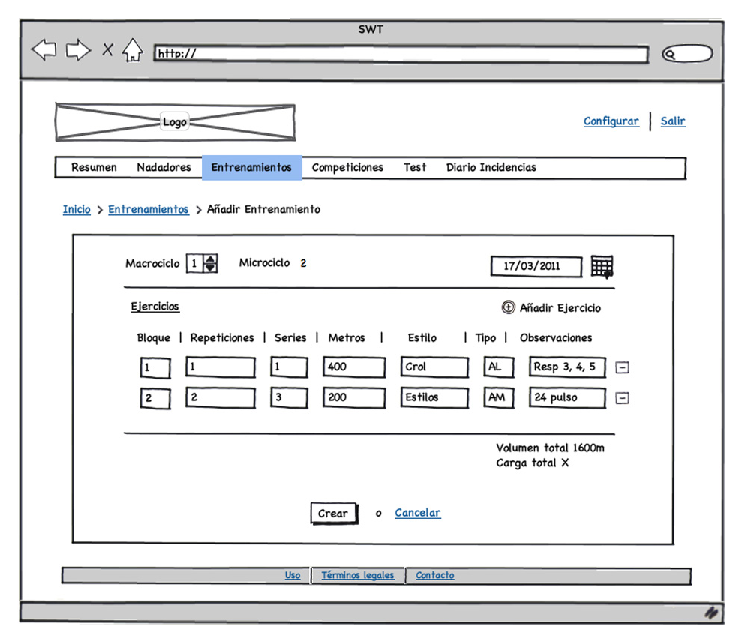
\includegraphics[width=8cm]{./eps/19_Entrenamientos_new.eps}
	  \caption{Interfaz para añadir entrenamiento}
	  \label{fig:interfaz_entrenamientos_new}
	\end{figure}

	% subsection gestión_de_entrenamientos (end)
% section diseño_de_interfaz_de_usuario (end)
% chapter análisis (end)